\documentclass[10pt,a4paper]{report}
\usepackage[utf8]{inputenc}
\usepackage{amsmath}
\usepackage{amsfonts}
\usepackage{amssymb}
\usepackage{graphicx}
\usepackage{hyperref}
\usepackage{tabto}
\usepackage{gensymb}
\usepackage{booktabs,caption,fixltx2e}
\usepackage[flushleft]{threeparttable}
\usepackage{tocloft}
\usepackage[margin=1in]{geometry}
\author{Finn Matras, Jakob Løver}
\title{{\LARGE TFY4115}\\{\large Friksjon på skråplan}}
\begin{document}
\renewcommand{\contentsname}{Innhold}
\renewcommand{\cftchapleader}{\cftdotfill{\cftdotsep}}
\renewcommand{\cftpartleader}{\cftdotfill{\cftdotsep}}

\maketitle
\tableofcontents
%\chapter*{Innhold}
%\begin{itemize}
%\item Sammendrag \tab{1}			
%\item Innledning \tab{2}
%\item Teori      \tab{3}
%\item Eksperimentelt \tab{4}
%\item Resultater og diskusjon \tab{5}
%\item Konklusjon \tab{6}
%\end{itemize}

\chapter*{Sammendrag}
\addcontentsline{toc}{chapter}{Sammendrag}
Formålet med laben var å regne seg frem til den horisontale vinkelen til et skråplan som gjør at et system bestående av to masser sklir med konstant hastighet. Friksjonskoeffisienten estimeres ved hjelp av Newtons II lov og videoanalyse-prgrammvaren Tracker. Målingene ble gjenntatt flere ganger for å verifisere og ta høyde for usikkerhet.\\
\\Kalkuleringene som ble foretatt viser til en friksjonskoeffisient mellom nylon og skråplanet i tre på 0.232 $\pm$ $0.026$, og 0.270 $\pm$ $0.020$ mellom plast og tre. Akselerasjonen som ble målt med vinkel $\theta = 12.4$ ga 0,02 $[m/s^2]$.

{\let\clearpage\relax\chapter*{Innledning}}
\addcontentsline{toc}{chapter}{Innledning}
I dette forsøket var formålet å bli kjent med hvordan en utfører eksperimentelle forsøk i fysikken, og å bli kjent med å skrive lab-journal og rapport. Ved hjelp av regresjoner av bevegelsen til en kloss som analyseres i Trasker kan en finne akselerasjonen, og så regne seg fram til friksjonskoeffisienten. Deretter settes det opp likninger for et massesystem og en kan regne ut vinkelen som fører til konstant hastighet.


{\let\clearpage\relax\chapter*{Teori}}
\addcontentsline{toc}{chapter}{Teori}
Basert på Newtons II lov som i likning (2): 
\begin{equation}
\sum{F} = m \cdot a,
\end{equation} der $F$ er kraften, $m$ er massen, og $a$ er akselerasjonen, så kan kreftene som er på en masse regnes ut. Likningen,
\begin{equation}
F_r = \mu \cdot F_n,
\end{equation}
der $F_r$ er friksjonskraften, $\mu$ er friksjonskoeffisienten, og $F_n$ er normalkraften til klossen på planet. 
\begin{equation}
F_x - F_r = m \cdot a,
\end{equation}
ved å sette opp likning (1) for Figur 3 fås likning (3). Ved hjelp av likning (2), kan likning (4) avledes,
\begin{equation}
\mu = \tan(\theta)-a/(\cos(\theta)\cdot g),
\end{equation}
$\theta$ er vinkelen mellom skråplanet og et horisontalt plan, $g$ er gravitasjonsakselerasjonen. Ved hjelp av denne liknignen kan en regne ut friksjonskoeffisienten for de forskjellige akselerasjonsmålingene. For å regne seg fram til vinkelen,$\theta$, mellom horisontalplanet og skråplanet, som gjør at massesystemet sklir med konstant fart ned langs skråplanet på et gitt underlag settes likning (1) opp for et system bestående av to masser, som vist i Figure \ref{oppsett}. Det antas her at de to massene er bunnet sammen med en masseløs snor, som forblir stram og at snorkreftene er like store.
\begin{equation}
F_{xm1} - F_{rm1} + F_{xm2} - F_{rm2} = m \cdot a,
\end{equation}
løser for vinkelen, $\theta$, der vi bruker $a = 0$, 
\begin{equation}
\theta = \arctan(\frac{\mu_1 \cdot m_1+\mu_2 \cdot m_2}{m_1+m_2}),
\end{equation}


\begin{figure}
der $m_1$ og $m_2$ er massene til klossene med tilhørende friksjonskoeffisienter $\mu_1$ og $\mu_2$.
\begin{center}
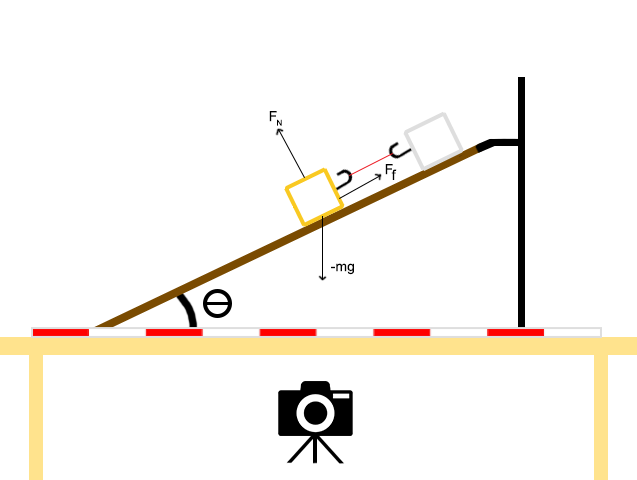
\includegraphics[scale=0.5]{withforces}
\caption{Illustrasjon av oppsettet, der $F_n$ er normalkraften fra skråplanet på klossen, $F_r$ er friksjonskraften mellom klossen og underlaget, og $-mg$ er gravitasjonskraften.}
\end{center}
\label{oppsett}
\end{figure}

For å finne middelverdien til de utregnede friksjonskoeffisientene ble likningen
\begin{equation}
\overline{\mu} = \dfrac{1}{n}\sum_{i=1}^{n}\mu_i
\end{equation}
 der $n$ er antall målinger, brukt. Videre ble usikkerheten i middelverdien regnet ut ved følgende likning,
\begin{equation}
\delta\overline{\mu} = \dfrac{\delta\mu}{\sqrt{n}}.
\end{equation}

\chapter*{Metoder og eksperiment}
\addcontentsline{toc}{chapter}{Metoder og eksperiment}
\section*{Metode}
\addcontentsline{toc}{section}{Metode}
\subsection*{Forberedelse}
\addcontentsline{toc}{subsection}{Forberedelse}
Et skjematisk oppsett av eksperimentet er vist i Figure \ref{oppsett}. Treplanken ble festet til et stativ med en klype. Det ble brukt vater for å påse at skråplanets vinkel blir målt normalt til tyngekraften. Foran oppsettet ligger det en meterstokk, noe som gjør det enkelt å kalibrere størrelsesforhold i programvaren Tracker. Høyhastighetskameraet er montert normalt på oppsettet, slik at vinkling på kameraet ikke påvirker størrelsene som måler. To forskjellige typer underlag ble brukt, som vist i Figure \ref{fig:1} og Figure \ref{fig:2}. De forskjellige underlagene ble festet på klosser av aluminium og messing ved hjelp av lærertyggis.\\
\\Som foreberedelse til laben ble likningene til laben utledet, beskrevet under seksjonen "Teori." Repetitive kalkulasjoner ble utført ved hjelp av et digital regneark. Innstillingene på høyhastighetskameraet ble tilpasset lysforholdene på laben. Dette resulterte i at det ble brukt 100fps med automatisk hvitbalanse.\\
\\En rekke eksperimenter ble fullført for å verifisere at utstyret fungerte. Ved hjelp av en vekt ble de to massenes vekt målt tre ganger. Gjennomsnittet av de tre målingene verifiserte at målingene var representative tall for vekten til massene. En av vektene ble sluppet foran en hvit vegg mens kameraet filmet. Dette filmklippet ble importert i Tracker. Ved hjelp av regresjonsfunksjonen i programmet ble integriteten til utstyret verifisert da denne gav 9.81 m/s$^2$ som akselerasjon.

\begin{figure}
    \centerline{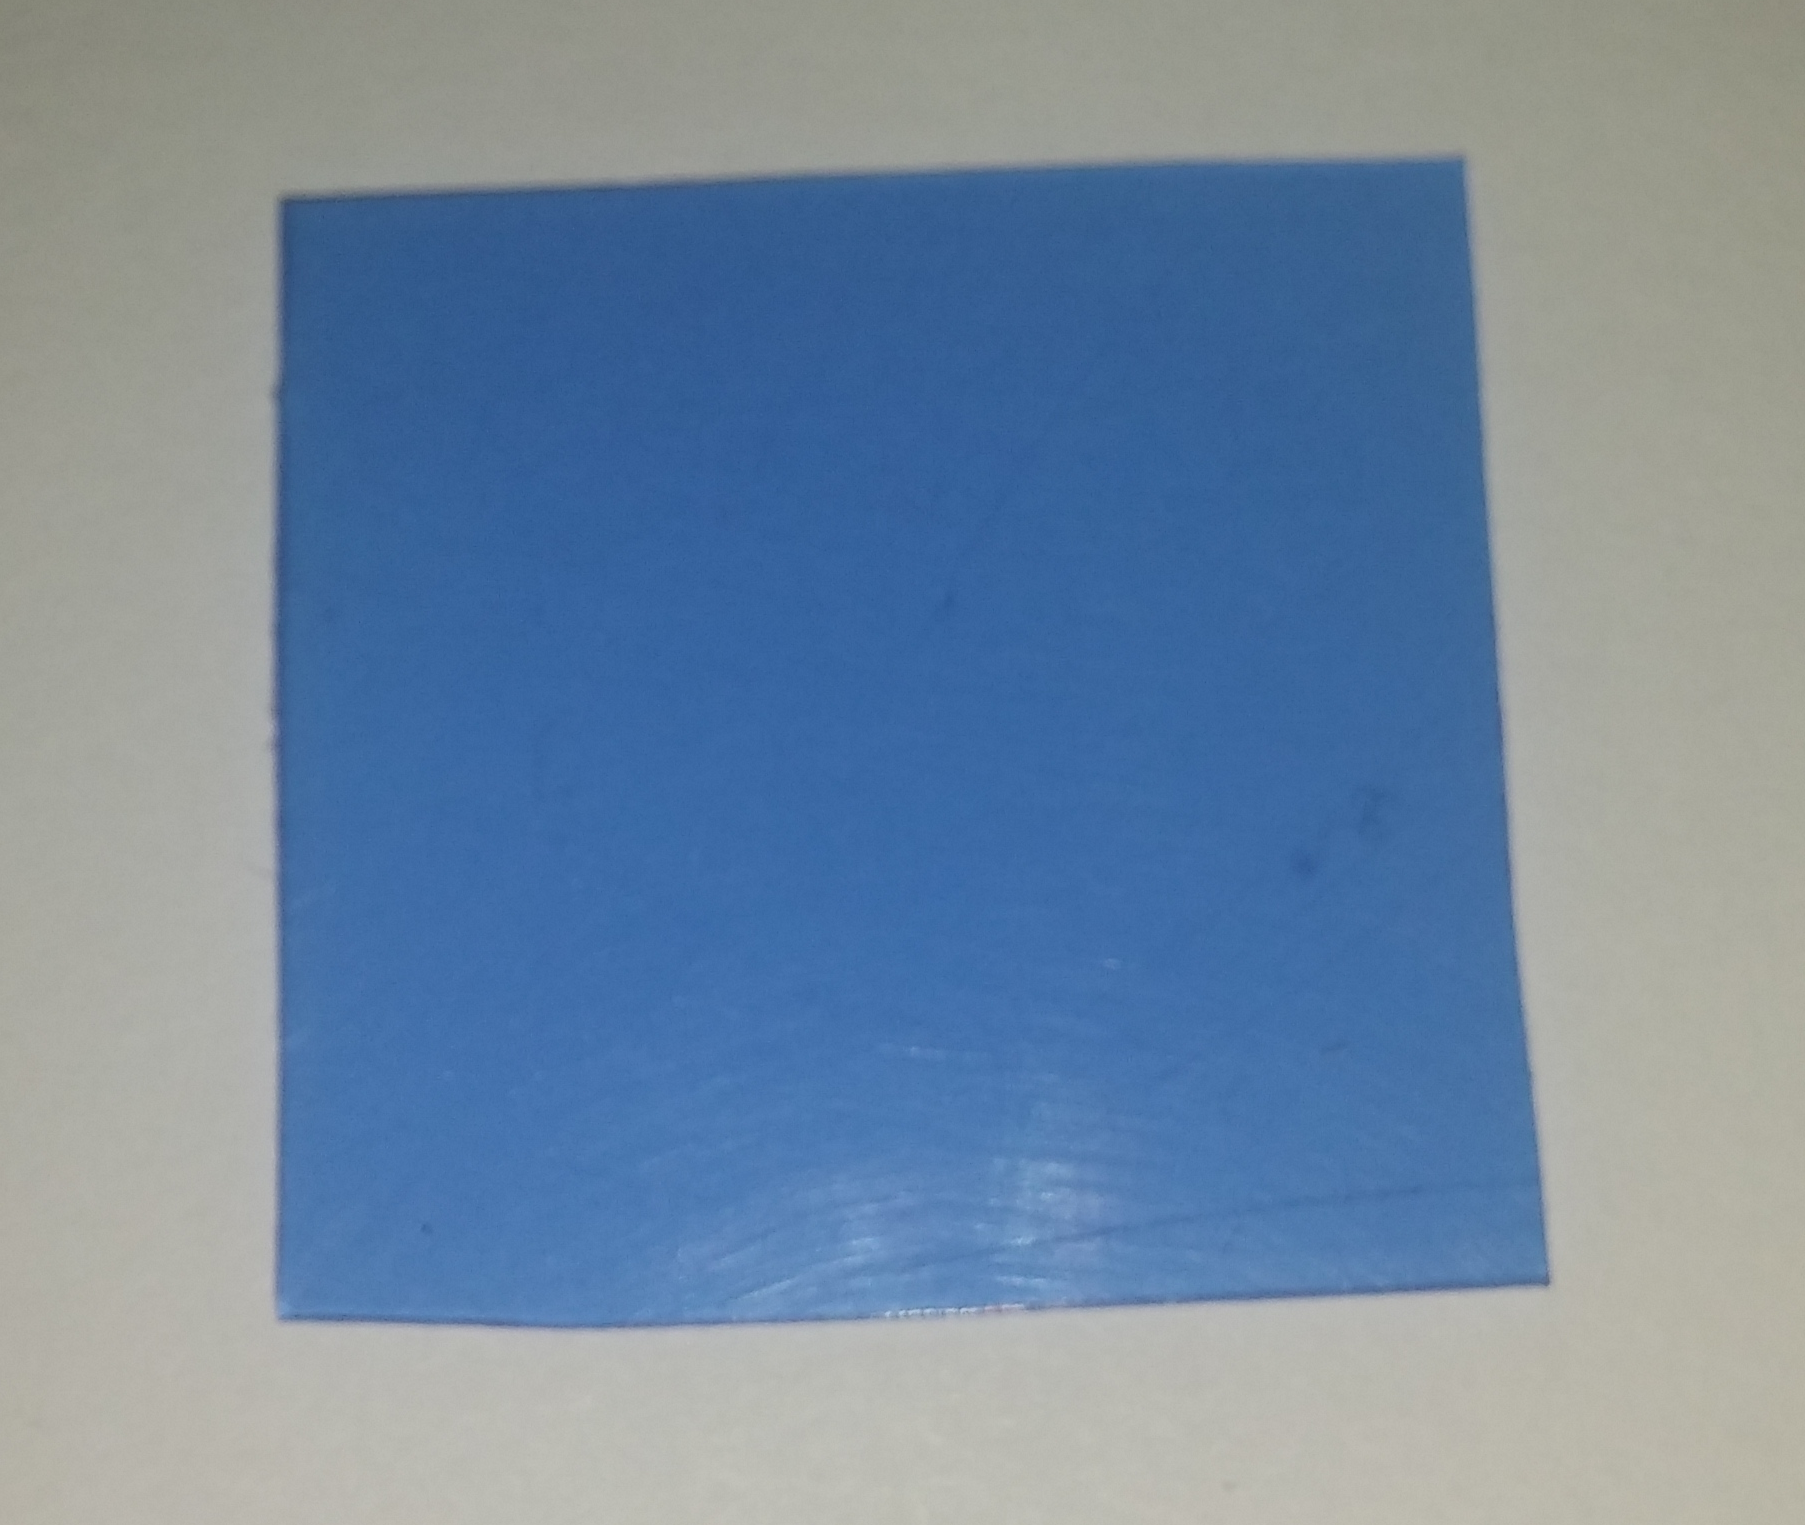
\includegraphics[scale=0.05]{BlaaPlast}}
    \caption{Blå plast, friksjonskoeffisient: 0.270.}
    \label{fig:1}
\end{figure}
\begin{figure}
    \centerline{\includegraphics[scale=0.05]{GultStoff}}
    \caption{Gul nylon, friksjonskoeffisient: 0.232.}
    \label{fig:2}
\end{figure}

\subsection*{Forsøk}
\addcontentsline{toc}{subsection}{Forsøk}
Forsøket ble gjennomført ved å først stille inn skråplanet til en vilkårlig vinkel. Med en linjal ble det tatt målinger av lengden og høyden av skråplanet, og brukte den inverse tangensen for å kalkulere vinkelen. Messingklossen ble sluppet 4 ganger nedover skråplanet, og importert i Tracker for å tilpasse akselerasjon. Ved hjelp av regnearket vårt og formlene definert ovenfor, ble friksjonskoeffesienten for klossen kalkulert. Dette ble gjentatt med aluminiumsklossen, og deretter med både nylonbiten og plastbiten som underlag. \\
\\De kalkulerte friksjonskoeffesientene for underlagene ble brukt til å beregne den vinkelen hvor begge klossene sklei ned med konstant hastighet. Klossene ble bundet sammen med en snor, og sluppet ned skråplanet. Tracker genererte en regresjon med en neglisjerbar akselerasjon, som bekreftet antagelsene. Dette gjøres med et gjenkjenningssystem i Tracker som automatisk gjenkenner klossene nedover skråplanet, og lager en punktgraf som kan brukes til å tilpasse en regresjon av typen andreordens polynom.\\
\\Til slutt ble optimal vinkel kalkulert med 10g vekter og 50g vekter lagt på hver av klossene. Da friksjonskoeffesientene var til underlagene var funnet i de forrige eksperimentene, ble vinkelen kalkuklert med de samme formlene. Denne gangen ble det også målt kun en neglisjerbar akselerasjon.


{\let\clearpage\relax\chapter*{Resultater og diskusjon}}
\addcontentsline{toc}{chapter}{Resultater og diskusjon}
\section*{Resultater}
\addcontentsline{toc}{section}{Resultater}
Nedenfor er resultatene som ble funnet ved å bruke Tracker til å finne akselerasjonen til klossene, ved hjelp av en regresjon av posisjonsgraf av bevegelsen til klossene. Vinkelen ble også funnet i Tracker, ved å se på vinkel mellom skråplanet og vateret. Tabell 1 viser målingene og tilhørende utregnede friksjonskoeffisienter, Tabell 2 viser gjennomsnittlige verdier for disse målingene med usikkerhet. Videre viser Tabell 3 den utregnede vinkelen $\theta$ som skal gi konstant hastighet for massesystemte ned skråplanet. Tabell 4 viser akselerasjonen for klossene med utregnet $\theta$, som teoretisk sett gir konstant hastighet, ingen akselerasjon.
\begin{center}
\begin{tablenotes}
 	\small
 	\item Tabell 1, viser rådata for akselerasjon og utregnet friksjonskoeffisient for klosstypene på oppgitt underlag, der det ble gjennomført fire målinger for hver kombinasjon av klosstype og underlag. Merk at for måling 13 til 16 ble vinkelen økt for å få klossen til å slik. Ellers ble samme vinkel brukt i de resterende målingene, men usikkerheten ligger i oppsettet av målingene i Tracker.
 	\end{tablenotes}
  \begin{tabular}{| c | c | c | c | c | c |}
    \hline
    Måling & Klosstype & Underlag & Akselerasjon $[m/s^2]$ & Vinkel [$^{\circ}$] & Friksjonskoeffisient \\ \hline
    1 & Messing & Nylon & 0.248 & 17.8 & 0.268 \\ \hline
    2 & Messing & Nylon & 0.412 & 16.9 & 0.216 \\ \hline
    3 & Messing & Nylon & 0.370 & 16.8 & 0.223 \\ \hline
    4 & Messing & Nylon & 0.366 & 16.7 & 0.222 \\ \hline
    5 & Aluminium & Nylon & 0.339 & 17.2 & 0.237 \\ \hline
    6 & Aluminium & Nylon & 0.299 & 16.8 & 0.238 \\ \hline
    7 & Aluminium & Nylon & 0.294 & 17.8 & 0.258 \\ \hline
    8 & Aluminium & Nylon & 0.306 & 17.5 & 0.250 \\ \hline
    9 & Messing & Plast & 0.337 & 18.2 & 0.256 \\ \hline
    10 & Messing & Plast& 0.196 & 18.7 & 0.296 \\ \hline
    11 & Messing & Plast& 0.296 & 17.8 & 0.258 \\ \hline
    12 & Messing & Plast& 0.189 & 18.2 & 0.288 \\ \hline
    13 & Aluminium & Plast & 0.431 & 25.0 & 0.369 \\ \hline
    14 & Aluminium & Plast & 0.418 & 24.9 & 0.370 \\ \hline
    15 & Aluminium & Plast & 0.572 & 26.1 & 0.360 \\ \hline
    16 & Aluminium & Plast & 0.766 & 25.3 & 0.300 \\ \hline
  \end{tabular}
\end{center}

Ved å bruke likning (7) og (8) ble så rådata omregnet til gjennomsnittlige verdier med usikkerhet.

\begin{center}
 \begin{tablenotes}
 	\small
 	\item Tabell 2, viser snitt for akselerasjon, vinkel og friksjonskoeffisient for de forskjellige underlagne og klossene med usikkerhet.
 	\end{tablenotes}
  \begin{tabular}{| c | c | c | c | c |}
    \hline
    Klosstype & Underlag & Akselerasjon $\pm$ $\delta A$ $[m/s^2]$ & Vinkel $\pm$ $\delta V$ [$^{\circ}$] & Friksjonskoeffisient $\pm$ $\delta \mu$ \\ \hline
    Messing & Nylon & 0.349 $\pm$ $0.082$ & 17.1 $\pm$ $0.6$ & 0.232 $\pm$ $0.082$ \\ \hline
    Aluminium & Nylon & 0.310 $\pm$ $0.023$ & 17.3 $\pm$ $0.5$ & 0.246 $\pm$ $0.086$\\ \hline
    Messing & Plast & 0.255 $\pm$ $0.074$ & 18.2 $\pm$ $0.5$ & 0.270 $\pm$ $0.095$\\ \hline
    Aluminium & Plast & 0.547 $\pm$ $0.174$ & 25.3 $\pm$ $0.6$ & 0.350 $\pm$ $0.126$\\ \hline
  \end{tabular}
\end{center}

Verdiene for gjennomsnittlig friksjonskoeffisient ble så satt inn i likning (6), for å få verdier for vinkelen, $\theta$, som skulle gi konstant hastighet for det sammensatte systemet.

\begin{center}
     \begin{tablenotes}
 	\small
 	\item Tabell 3, viser vinkelen, $\theta$ som teoretisk sett skal gi konstant hastighet ned skråplanet, med usikkerhet.
 	\end{tablenotes}
  \begin{tabular}{| c | c | c |}
    \hline
    Stoff kloss 1 & Stoff kloss 2 & $\overline{\theta} \pm \delta\theta$ \\ \hline
    Nylon & Nylon & 13.6 $\pm$ 0.8 \\ \hline
    Plast & Plast & 16.4 $\pm$ 1.2 \\ \hline
    Nylon & Plast & 17.7 $\pm$ 1.7 \\ \hline
    Plast & Nylon & 14.7 $\pm$ 1.5  \\ \hline
  \end{tabular}
\end{center}
Tabellen nedenfor viser at dersom en tok den minste vinkelen som var innenfor usikkerheten, så ble akselerasjonen til systemet nesten lik null.

\begin{center}
     \begin{tablenotes}
 	\small
 	\item Tabell 4, viser resultatene fra målingene som ble gjennomført på klosser med gitt vekt og utregnet friksjonskoeffisient og vinkel for konstant hastighet, altså ingen akselerasjon. 
 	\end{tablenotes}
  \begin{tabular}{| c | c | c | c | c  | c |}
    \hline
    Underlag kloss 1 & Underlag kloss 2 & Vekt kloss 1 [kg] & Vekt kloss 2 [kg] & Vinkel $\theta$ & Akselerasjon $[m/s^2]$ \\ \hline
    Nylon & Nylon & 0.022 & 0.0687 & 12.8 & 0.12 \\ \hline
    Nylon & Plast & 0.0242 & 0.0687 & 16.0 & 0.02 \\ \hline
    Plast & Nylon & 0.0343 & 0.1197 & 13.3 & 0.04 \\ \hline
    Plast & Plast & 0.0343 & 0.1197 & 16.0 & lav, mistet data  \\ \hline
  \end{tabular}
\end{center}


\section*{Diskusjon og feilkilder}
\addcontentsline{toc}{section}{Diskusjon og feilkilder}
Som en ser i resultatene ovenfor, så ga alle de teoretisk utregnede verdiene en vinkel som var for stor, noe som førte til at klossene akselererte nedover skråplanet. En feilkilde som ble observert mens testene ble gjennomført var at klossene beveget seg litt hakkete nedover skråplanet. Dette er høyst sannsynlig forårsaket ved at skråplanet ikke har helt homogen overflate, noe som gjør at friksjonskoeffisientene endrer seg nedover langs skråplanet. Klossene ble ikke alltid sluppet på akuratt samme sted, da skråplanet var forholdsvis bredt, og overflaten kan også være forskjellig i bredden, noe som kan ha forårsaket feil i målingne. Ut ifra likning (3) ser en også at vinkelen, $\theta$ har mye å si, dette ble også observert ved de initielle målingene. At vateret ble brukt til å finne nøyaktig horisontal posisjon var svært viktig, men her kan det fortsatt være noe usikkerhet, med tanke på hvordan det ble overført til Tracker.\\\\
Måling 13 til og med 16 i Tabell 1, gir større verdier for friksjonskoeffisienten enn målingene 9 til 12 i samme tabell. Det ble også observert at klossen i måling 13 til 16 hadde høyere hastighet. Her er både klossen og vinkelen endret. Vel å merke her er at det er forskjell på friksjon avhengig av hastighet mellom de to underlagene. Det vil si at det for plasten var en annen friksjonskoeffisient ved høyere hastigheter enn ved lavere hastigheter. Fordi resultatene viser at friksjonskoeffisienten endrer seg med hastigheten, og formålet er å finne friksjonskoeffisienten ved konstant hastighet, så kunne det vært lurt å utføre målingene med så jevn hastighet som mulig, for at friksjonskoeffisienten skal være så lik som mulig det den er ved konstant hastighet. Etter å ha sammenliknet friksjonskoeffisienten for metall og tre, som ble målt initielt, med verdier funnet på internett [1], kan en konkludere med at målingene for friksjonskoeffisientene ligger innenfor det område som kan forventes.\\\\
En annen ting som ble observert i målingene som ble gjennomført helt i starten av en kloss i fritt fall, var at selv om klossen falt fritt, så stemte ikke alltid akselerasjonsverdiene som ble funnet i Tracker. Verdiene for gravitasjonsakselerasjonen lå i nærheten av det en skulle forvente, men at verdiene hadde en usikkerhet på rundt $\pm$ 20$\%$. Derfor ble det tatt totalt 8 målinger av hver stofftype, men for enda mer presise resultater kunne det blitt gjort en rekke flere målinger.

{\let\clearpage\relax\chapter*{Konklusjon}}
\addcontentsline{toc}{chapter}{Konklusjon}
Hypotesen vår var at det var mulig å finne en optimal vinkel for konstant hastighet for et massesystem med gitt underlag, noe som kan konkluderes med at ble oppnådd, da hastigheten var nesten konstant, med akselerasjoner på mellom 0.12 $[m/s^2]$ til 0.02 $[m/s^2]$. Det var en del feilkilder som gjorde at resultatene våre ikke ble slik som forventet, dette gjelder blandt annet uhomogen overflate på skråplanet, regresjon i Tracker og unøyaktigheter i oppsett av måling i Tracker. Det opplevdes ofte at den kalkulerte vinkelen var for høy.

\chapter*{Referanser}
[1] \href{url}{https://en.wikipedia.org/wiki/Friction}
Nedlastingsdato: 26. oktober 2016

\end{document}

